\documentclass[utf8]{FrontiersinHarvard}

\usepackage{url,hyperref,microtype}
\usepackage{svg}
\usepackage{graphicx}
\usepackage{amssymb}
\usepackage[default]{sourcesanspro}

% Use one contemporary sans-serif family throughout the document.
\renewcommand{\familydefault}{\sfdefault}
\renewcommand{\helvetica}{\sffamily}
\renewcommand{\helveticaitalic}{\sffamily\itshape}
\renewcommand{\helveticabold}{\sffamily\bfseries}
\renewcommand{\helveticabolditalic}{\sffamily\bfseries\itshape}

% Match figure artwork to the bordered, lightly shaded abstract panel.
\newcommand{\boxedfigure}[1]{%
  \fcolorbox{BorderGray}{LightBg}{%
    \begin{minipage}{0.94\linewidth}
      \centering
      #1
    \end{minipage}}}

% Permit comfortable wrapping in the narrow journal columns.
\tolerance=2000
\hyphenpenalty=200
\exhyphenpenalty=50
\setlength{\emergencystretch}{2em}
\newcommand{\breakslash}{/\penalty0\hspace{0pt}}

\title{Feasibility of Matrix-Coprocessor Acceleration for Post-Quantum Cryptography on Apple Silicon: From Saber\breakslash FrodoKEM to ML-KEM, MAYO, HQC, and NTRU~Prime}

\def\firstAuthorLast{Singh}
\def\Address{Department of Computer Science and Engineering (Cybersecurity), Vellore Institute of Technology, Chennai, India}
\def\corrAuthor{Diljot Singh}
\def\corrEmail{diljot.singh2024@vitstudent.ac.in}

\author[Singh]{Diljot Singh}
\address{}
\correspondance{}
\extraAuth{}

\begin{document}

\maketitle

\begin{abstract}
\section{}
Apple's undocumented AMX matrix coprocessor has been shown to accelerate two lattice-based post-quantum KEMs --- Saber (via Toeplitz Matrix-Vector Product reformulations of polynomial arithmetic) and FrodoKEM (via direct matrix multiplication and \texttt{GENLUT}-assisted sampling) --- on Apple M1 and M3 SoCs~\cite{gazzoni2024pqcamx}. This paper investigates whether AMX acceleration generalizes beyond these two schemes by evaluating four additional post-quantum primitives that span fundamentally different algebraic workloads: \textbf{ML-KEM} (FIPS~203~\cite{fips203}), the NIST-standardized lattice KEM using NTT-domain polynomial arithmetic over $\mathbb{Z}_{3329}$; \textbf{MAYO}~\cite{mayo2025spec}, a NIST Round~2 additional multivariate signature candidate evaluating dense quadratic forms over $\mathbb{F}_{16}$; \textbf{HQC}~\cite{hqc2025spec}, a recently selected code-based KEM performing polynomial multiplication over $\mathbb{F}_2$; and \textbf{Streamlined NTRU~Prime}~\cite{ntruprime2017spec} (\texttt{sntrup761}), a lattice KEM using a non-NTT-friendly ring $\mathbb{Z}_{4591}[x]/(x^{761}-x-1)$.

We implement AMX-accelerated arithmetic kernels for all four schemes on Apple M3, alongside ARM NEON baselines, and report cycle-accurate and wall-clock measurements. Throughout, we define kernel speedup as $S = t_{\text{NEON}} / t_{\text{AMX}}$, where $S > 1$ indicates AMX is faster. Our key findings establish a \emph{suitability heuristic}: AMX kernel acceleration tends to provide speedup when the computational bottleneck is a dense integer multiply-accumulate over a small modulus without a competing dedicated NEON instruction. For the isolated kernels tested, MAYO achieves $S$ up to $1.69$ (MAYO-5), and the \texttt{sntrup761} ternary-by-dense product achieves $S = 1.52$. Conversely, ML-KEM's isolated polynomial multiplication kernel shows $S \approx 0.013$ (a ${\sim}75\times$ slowdown) because NEON NTT butterfly operations dominate, and HQC's dense multiplication kernel shows $S \approx 0.0006$ (a ${\sim}1{,}562\times$ slowdown) because NEON carry-less multiply (\texttt{PMULL}) is purpose-built for $\mathbb{F}_2$ arithmetic that AMX cannot perform.

\abstractkeywords{Apple AMX; post-quantum cryptography; matrix coprocessor; ML-KEM; MAYO; HQC; NTRU Prime; NEON; NTT; hardware acceleration}
\end{abstract}

% =============================================================
\section{Introduction}

The transition from classical to post-quantum cryptography has produced a diverse ecosystem of schemes built upon lattices, codes, multivariate polynomials, hash functions, and isogenies~\cite{nist2022pqc}. As these schemes move toward deployment, optimized implementations on commodity hardware become critical~\cite{nejatollahi2019pqcsurvey}. Modern system-on-chip (SoC) processors contain specialized coprocessors --- SIMD engines, matrix accelerators, and cryptographic extensions --- that can dramatically affect the performance landscape.

Apple's M-series SoCs include an undocumented matrix coprocessor known as AMX (Apple Matrix eXtensions)~\cite{dougallj2022amx}. AMX provides a $32\times32$ integer multiply-accumulate engine operating on a dedicated 4~KB Z register file, with 64-byte X and Y input registers. Gazzoni Filho et al.~\cite{gazzoni2024pqcamx} demonstrated that AMX can accelerate the polynomial multiplication bottleneck of Saber~\cite{dangelo2018saber} (up to 13\% kernel speedup via TMVP reformulation) and the matrix-multiplication and sampling bottleneck of FrodoKEM~\cite{bos2020frodokem} (up to 21\% kernel speedup via direct matrix products and \texttt{GENLUT}-assisted noise sampling).

However, Saber and FrodoKEM share specific algebraic properties that make them amenable to AMX: both use power-of-two moduli ($q = 2^{13}$ for Saber), enabling free mod-$2^{16}$ overflow in AMX's 16-bit accumulators, and neither uses Number Theoretic Transforms (NTTs). The generalizability of AMX acceleration to the broader post-quantum landscape --- especially to NTT-based schemes, multivariate schemes, code-based schemes, and non-cyclotomic lattice schemes --- remained an open question.

This paper systematically investigates this question by implementing and benchmarking isolated arithmetic kernels for four post-quantum primitives on Apple M3, spanning four distinct algebraic workload classes:

\begin{enumerate}
  \item \textbf{ML-KEM (FIPS~203)~\cite{fips203}}: NTT-based polynomial multiplication over $\mathbb{Z}_{3329}[x]/(x^{256}+1)$.
  \item \textbf{MAYO~\cite{mayo2025spec}}: Dense multivariate quadratic form evaluation over $\mathbb{F}_{16}$, a non-NTT workload.
  \item \textbf{HQC~\cite{hqc2025spec}}: Polynomial multiplication over $\mathbb{F}_2[x]/(x^n - 1)$, a binary-field code-based KEM.
  \item \textbf{Streamlined NTRU~Prime~\cite{ntruprime2017spec} (\texttt{sntrup761})}: Polynomial multiplication over $\mathbb{Z}_{4591}[x]/(x^{761}-x-1)$, a non-NTT-friendly non-cyclotomic lattice ring with prime modulus.
\end{enumerate}

We define kernel speedup as $S = t_{\text{NEON}} / t_{\text{AMX}}$ throughout; $S > 1$ means AMX is faster for the measured kernel. Our results establish a \emph{suitability heuristic} for AMX acceleration of post-quantum workloads (summarized in Figure~\ref{fig:crossscheme}) and reveal two novel AMX implementation techniques: bounded Z-register accumulation for prime moduli (NTRU~Prime), and the critical register-zero invariant required by the \texttt{MAC16\_Y\_SKIP} hardware instruction.


% =============================================================
\section{Summary of the Base Paper}
\label{sec:basepaper}

Gazzoni Filho et al.~\cite{gazzoni2024pqcamx} present PQC-AMX, an acceleration framework for Saber and FrodoKEM on Apple M1 and M3 SoCs using the AMX matrix coprocessor. Their contributions decompose into two distinct workload mappings:

\subsection{AMX Architecture}

AMX is a CPU-coupled matrix-multiply engine present in all Apple Silicon since the A13 Bionic~\cite{dougallj2022amx}. It maintains a private register file comprising eight 64-byte X registers, eight 64-byte Y registers, and a $64\times64$-byte Z register (4~KB total), as illustrated in Figure~\ref{fig:amx-registers}. The primary computational primitive is \texttt{mac16}, which computes a $32\times32$ outer product of 16-bit integer vectors from X and Y, accumulating results into Z:
\[
  Z[r][c] \mathrel{+}= X[r] \times Y[c], \quad r, c \in [0, 31].
\]

The Z register is persistent across \texttt{mac16} calls, enabling multi-step accumulation. A \texttt{Z\_SKIP} flag clears Z before the multiplication. AMX also provides \texttt{EXTRH} (extract horizontal --- copy Z rows to X/Y registers with lane shifting), \texttt{VECINT} (vector integer add/shift), and \texttt{GENLUT} (generalized lookup table for finite-field arithmetic)~\cite{corsix2022amx}. AMX operates as a coprocessor on the CPU's data path; it is activated via \texttt{AMX\_SET()} and deactivated via \texttt{AMX\_CLR()}, and is thread-local.

\begin{figure}[htbp]
  \centering
  \boxedfigure{\includesvg[width=\linewidth,inkscapelatex=false]{amx-register-layout}}
  \caption{Organization of the AMX register file (X, Y, Z) and the $32\times32$ outer-product multiply-accumulate primitive. Each X/Y register holds 32 lanes of 16-bit integers (64 bytes), and the Z register stores the accumulated outer product.}
  \label{fig:amx-registers}
\end{figure}

\subsection{Saber: TMVP Reformulation of Polynomial Arithmetic}

For Saber~\cite{dangelo2018saber}, the authors reformulate polynomial multiplication in the ring $\mathbb{Z}_q[X]/(X^n+1)$ as a Toeplitz Matrix-Vector Product (TMVP)~\cite{toeplitz1911theorie}. The polynomial product $c = a \cdot b$ is decomposed into block outer products of 32-coefficient slices, with anti-diagonal extraction (via \texttt{EXTRH}/\texttt{VECINT}) recovering the convolution coefficients entirely within AMX registers. For Saber ($q = 2^{13}$, $n = 256$), this requires $8 \times 8 = 64$ \texttt{mac16} outer products, with the mod-$2^{13}$ reduction obtained for free from the 16-bit register wrapping (since $2^{13} \mid 2^{16}$).

\subsection{FrodoKEM: Matrix Multiplication and GENLUT Sampling}

For FrodoKEM~\cite{bos2020frodokem}, the workload is fundamentally different: it involves dense matrix-matrix and matrix-vector products over $\mathbb{Z}_q$ (with $q$ up to $2^{16}$), which map directly to AMX's \texttt{mac16} without TMVP reformulation. Additionally, the authors exploit AMX's \texttt{GENLUT} instruction to sample discrete Gaussian noise in constant time using table lookups.

\subsection{Reported Results}

On Apple M3, the authors report kernel speedups of up to 13\% ($S = 1.13$) for Saber's polynomial arithmetic and up to 21\% ($S = 1.21$) for FrodoKEM's matrix operations over optimized ARM NEON baselines~\cite{gazzoni2024pqcamx}. They explicitly note that NTT-based schemes and non-lattice primitives remain unexplored.


% =============================================================
\section{Research Gap and Motivation}
\label{sec:gap}

The base paper establishes AMX's viability for two specific schemes but leaves several critical questions unanswered:

\begin{enumerate}
  \item \textbf{NTT-amortized schemes (ML-KEM).} ML-KEM stores public and secret keys in the NTT domain, amortizing the $O(n \log n)$ forward transform~\cite{longa2016speeding}. Whether the $O(n^2)$ AMX TMVP schoolbook approach can compete with NEON's $O(n \log n)$ NTT butterfly pipeline, even considering AMX's higher per-instruction throughput, is unknown.
  
  \item \textbf{Non-lattice multivariate schemes (MAYO).} MAYO evaluates dense quadratic forms $y_k = \mathbf{x}^T P_k \mathbf{x}$ over $\mathbb{F}_{16}$~\cite{beullens2022mayo}, a workload that is structurally similar to matrix multiplication but operates over 4-bit nibbles rather than 16-bit integers. AMX's \texttt{GENLUT} instruction provides finite-field lookup capability, but its utility for $\mathbb{F}_{16}$ matrix-vector products has not been evaluated.
  
  \item \textbf{Binary-field code-based schemes (HQC).} HQC performs polynomial multiplication over $\mathbb{F}_2$, where the arithmetic is carry-less (XOR-based)~\cite{hqc2025spec}. AMX provides \emph{integer} multiply-accumulate with carries, and lacks native bitwise XOR/AND operations, raising the question of whether AMX can be useful for $\mathbb{F}_2$ workloads at all.
  
  \item \textbf{Non-NTT lattice schemes with prime moduli (NTRU~Prime).} \texttt{sntrup761} deliberately uses a non-cyclotomic ring $\mathbb{Z}_{4591}[x]/(x^{761}-x-1)$ that is algebraically incompatible with NTT~\cite{ntruprime2017spec}. Its prime modulus $q = 4591$ does not divide $2^{16}$, preventing the free overflow exploitation that Saber enjoyed.
  
  \item \textbf{Apple M3 characterization.} No prior work has published cycle-count or wall-clock measurements for any of these four schemes using AMX on Apple M3 hardware.
\end{enumerate}

The NTT-based multiplication approach used by ML-KEM is illustrated in Figure~\ref{fig:ntt-butterfly}, contrasting the $O(n \log n)$ butterfly structure with the $O(n^2)$ schoolbook/TMVP approach mapped to AMX.

\begin{figure}[htbp]
  \centering
  \boxedfigure{\includesvg[width=\linewidth,inkscapelatex=false]{fft-butterfly}}
  \caption{Comparison of $O(n\log n)$ NTT butterfly multiplication (used by ML-KEM) versus the $O(n^2)$ schoolbook/TMVP matrix outer-product approach mapped onto AMX. The NTT stores keys in pre-transformed domain, amortizing the forward transform cost.}
  \label{fig:ntt-butterfly}
\end{figure}


% =============================================================
\section{Problem Statement}

Given that Apple AMX accelerates Saber's polynomial arithmetic and FrodoKEM's matrix operations via distinct reformulations~\cite{gazzoni2024pqcamx}, under what algebraic conditions does AMX kernel acceleration remain beneficial for post-quantum cryptographic schemes? Specifically, this paper asks:

\begin{enumerate}
  \item Does AMX's $O(n^2)$ TMVP approach provide a net kernel performance gain over NEON's $O(n \log n)$ NTT pipeline for the NIST-standardized ML-KEM?
  \item Can AMX's matrix and lookup-table primitives accelerate MAYO's dense $\mathbb{F}_{16}$ quadratic form evaluation kernel?
  \item Can AMX accelerate the $\mathbb{F}_2$ polynomial multiplication kernel for the code-based KEM HQC?
  \item Can AMX accelerate the polynomial multiplication kernel for NTRU~Prime's non-NTT-friendly prime-modulus ring?
  \item What structural properties of a post-quantum scheme's arithmetic kernel determine whether AMX acceleration is feasible?
\end{enumerate}


% =============================================================
\section{Contributions}

This paper makes the following contributions:

\begin{enumerate}
  \item \textbf{Four new AMX kernel implementations.} We implement AMX-accelerated arithmetic kernels for ML-KEM (all parameter sets: 512/768/1024), MAYO (all parameter sets: 1/2/3/5), HQC-128, and \texttt{sntrup761} on Apple M3.
  
  \item \textbf{Empirical suitability heuristic.} Through benchmarking of isolated kernels, we observe that AMX tends to provide kernel speedup when the computational bottleneck is a dense integer multiply-accumulate over a modulus fitting in 16-bit AMX lanes, and no dedicated NEON instruction (NTT butterfly, carry-less \texttt{PMULL}) exists for the operation. We note that this heuristic is derived from six data points and should be treated as a working hypothesis rather than a universal law.
  
  \item \textbf{Two novel AMX techniques.}
  \begin{itemize}
    \item \emph{Bounded Z-accumulation for prime moduli}: For NTRU~Prime ($q = 4591$), we group block pairs on the same anti-diagonal and accumulate $\leq 7$ \texttt{mac16} outer products per Z flush, keeping partial sums within signed 16-bit range ($7 \times 4590 = 32{,}130 < 32{,}768$).
    \item \emph{Register-zero invariant}: We document that AMX's \texttt{MAC16\_Y\_SKIP} instruction implicitly uses \texttt{Y\_REG(0)} as its Y operand, requiring \texttt{X\_REG(0)} and \texttt{Y\_REG(0)} to be loaded with zeroes throughout the anti-diagonal extraction (flatten) procedure. Input data must be loaded into \texttt{X\_REG(1)} and \texttt{Y\_REG(1)} or higher.
  \end{itemize}
  
  \item \textbf{Benchmark dataset.} We report measurements on Apple M3 for all four schemes' arithmetic kernels, providing the first published AMX performance characterization for ML-KEM, MAYO, HQC, and NTRU~Prime kernels. We note that these are subroutine-level measurements and do not represent full protocol performance.
\end{enumerate}


% =============================================================
\section{Background and Preliminaries}
\label{sec:background}

\subsection{ML-KEM (FIPS~203)}

ML-KEM~\cite{fips203} operates over the polynomial ring $R_q = \mathbb{Z}_{3329}[x]/(x^{256}+1)$. The cyclotomic polynomial $x^{256}+1$ admits a Number Theoretic Transform (NTT) over $\mathbb{Z}_{3329}$, since $3329$ is prime and $256 \mid (3329-1)$~\cite{longa2016speeding}. Polynomial multiplication in ML-KEM is therefore computed as:
\[
  c = \text{NTT}^{-1}(\text{NTT}(a) \circ \text{NTT}(b)),
\]
where $\circ$ denotes coefficient-wise multiplication in the NTT domain. Crucially, ML-KEM stores public and secret keys in NTT-domain representation, amortizing the forward NTT cost across operations. This means that the polynomial multiply bottleneck reduces to a single inverse NTT plus coefficient-wise products, each of which is $O(n \log n)$ with small constants on NEON~\cite{becker2022neon}.

\subsection{MAYO Signature Scheme}

MAYO~\cite{mayo2025spec,beullens2022mayo} is a multivariate signature scheme based on the Oil-and-Vinegar (UOV) construction~\cite{kipnis1999uov}. Its signing operation evaluates $m$ quadratic forms:
\[
  y_k = \mathbf{x}^T P_k \mathbf{x}, \quad k = 1, \ldots, m,
\]
where $P_k$ are $n \times n$ matrices over $\mathbb{F}_{16}$ and $\mathbf{x} \in \mathbb{F}_{16}^n$. For MAYO-1, $(m, n) = (64, 66)$; for MAYO-5, $(m, n) = (128, 133)$. The arithmetic over $\mathbb{F}_{16} = \mathbb{F}_2[\alpha]/(\alpha^4 + \alpha + 1)$ requires multiplication via lookup tables or carry-less operations, with no NTT structure. Note: these are the Round~2 parameter sets~\cite{mayo2025spec}; we benchmark the quadratic form evaluation kernel at these dimensions.

\subsection{HQC (Hamming Quasi-Cyclic)}

HQC~\cite{hqc2025spec} is a code-based KEM recently selected by NIST as the fifth post-quantum standard~\cite{nist2025hqc}. It operates over $\mathbb{F}_2[x]/(x^n - 1)$ with $n = 17{,}669$ for HQC-128. Its bottleneck is polynomial multiplication over $\mathbb{F}_2$, where all coefficient arithmetic is carry-less (XOR for addition, AND-with-shift for multiplication). ARM NEON provides the \texttt{PMULL} instruction for hardware-accelerated carry-less multiplication of 64-bit operands~\cite{arm2021neon}.

\subsection{Streamlined NTRU~Prime (\texttt{sntrup761})}

Streamlined NTRU~Prime~\cite{ntruprime2017spec} operates over $\mathbb{Z}_{4591}[x]/(x^{761} - x - 1)$. The non-cyclotomic polynomial $x^{761} - x - 1$ was chosen specifically to resist certain algebraic attacks enabled by cyclotomic structure. The prime modulus $q = 4591$ fits in 13 bits ($4591 < 2^{13}$) but does not divide $2^{16}$, precluding the free overflow technique used for Saber~\cite{dangelo2018saber}. The KEM bottleneck involves multiplying a ternary polynomial $r \in \{-1, 0, 1\}^{761}$ by a general polynomial $h \in \mathbb{Z}_{4591}^{761}$.


% =============================================================
\section{Methodology}
\label{sec:methodology}

For each scheme, we follow the four-stage pipeline illustrated in Figure~\ref{fig:methodology}:

\begin{figure}[htbp]
  \centering
  \boxedfigure{\includesvg[width=\linewidth,inkscapelatex=false]{methodology-blocks}}
  \caption{Four-stage methodology pipeline: baseline acquisition, AMX reformulation, integration, and benchmarking with iterative feedback from Stage~4 to Stage~2.}
  \label{fig:methodology}
\end{figure}

\textbf{Stage~1: Baseline acquisition.} We obtain reference C and optimized ARM NEON implementations. For ML-KEM, we use the \texttt{neon-ntt} library~\cite{becker2022neon} for Cooley--Tukey NTT butterflies. For HQC, we implement NEON carry-less multiplication using \texttt{PMULL}/\texttt{PMULL2}~\cite{arm2021neon}. For NTRU~Prime, we implement NEON widening multiply-accumulate (\texttt{vmlal\_s16}). For MAYO, we implement NEON-based nibble lookup for $\mathbb{F}_{16}$ arithmetic.

\textbf{Stage~2: AMX reformulation.} We map each scheme's computational bottleneck to AMX primitives:
\begin{itemize}
  \item ML-KEM: TMVP reformulation of polynomial multiply using \texttt{mac16} outer products (following the base paper's Saber approach~\cite{gazzoni2024pqcamx}).
  \item MAYO: Quadratic form evaluation using \texttt{mac16} matrix mode and \texttt{GENLUT} for $\mathbb{F}_{16}$ multiplication tables.
  \item HQC: Integer-encoded $\mathbb{F}_2$ polynomial multiplication (each bit stored as a 16-bit lane value 0 or 1) with \texttt{mac16} outer products.
  \item NTRU~Prime: TMVP with bounded Z-accumulation (groups of $\leq 7$ \texttt{mac16} outer products) and 32-bit software anti-diagonal extraction.
\end{itemize}

\textbf{Stage~3: Integration.} Each AMX kernel is integrated into a test harness with the reference and NEON implementations, compiled with Apple Clang \texttt{-O3} on macOS.

\textbf{Stage~4: Benchmarking.} We measure performance using two methods: (a)~hardware cycle counts via \texttt{kperf} performance counters for ML-KEM full-operation benchmarks, and (b)~wall-clock time via \texttt{std::chrono::high\_resolution\_clock} for isolated kernel benchmarks (MAYO, HQC, NTRU~Prime). We report median values over $\geq 20$ iterations after warmup. All measurements are performed on Apple M3 (MacBook Air, 8-core, macOS Sequoia 15) with the process pinned to performance cores. The M3 performance cores operate at a nominal frequency of 4.05~GHz; cycle-to-microsecond conversions use $1~\mu\text{s} \approx 4{,}050$~cycles. We do not report confidence intervals; variance across runs was consistently below 3\%.


% =============================================================
\section{Implementation Details}
\label{sec:implementation}

\subsection{ML-KEM: TMVP vs.\ NTT}

We implement the TMVP-based polynomial multiplication from the base paper~\cite{gazzoni2024pqcamx}, adapted for ML-KEM's ring $\mathbb{Z}_{3329}[x]/(x^{256}+1)$. The polynomial degree $n = 256$ yields $\lceil 256/32 \rceil = 8$ blocks, requiring $8 \times 8 = 64$ \texttt{mac16} outer products.

\textbf{Key obstacle:} ML-KEM's modulus $q = 3329$ is prime and does not divide $2^{16}$, so the mod-$2^{16}$ accumulation used for Saber is incorrect. More fundamentally, the NEON NTT baseline benefits from \emph{domain amortization}~\cite{longa2016speeding}: public and secret keys are stored in NTT form, so each polynomial multiplication requires only a coefficient-wise multiply plus a single inverse NTT, amortizing the forward transform cost. The AMX TMVP operates in the coefficient domain and cannot exploit this amortization.

\subsection{MAYO: $\mathbb{F}_{16}$ Quadratic Forms via GENLUT}

MAYO's bottleneck is the evaluation of $m$ quadratic forms $y_k = \mathbf{x}^T P_k \mathbf{x}$ over $\mathbb{F}_{16}$~\cite{beullens2022mayo}. We map this to AMX as follows:

\begin{enumerate}
  \item Pack four $\mathbb{F}_{16}$ elements per 16-bit lane (4 bits each).
  \item Use AMX \texttt{GENLUT} to perform $\mathbb{F}_{16}$ multiplication via precomputed lookup tables stored in AMX registers.
  \item Accumulate partial inner products in the Z register.
\end{enumerate}

This approach achieves high throughput because MAYO's quadratic form evaluation is inherently a dense matrix-vector product with no NTT competitor.

\subsection{HQC: $\mathbb{F}_2$ via Integer Encoding}

Since AMX has no native bitwise XOR/AND operations~\cite{corsix2022amx}, we encode each $\mathbb{F}_2$ element as a 16-bit integer (0 or 1). Polynomial multiplication over $\mathbb{F}_2$ then becomes integer convolution modulo 2: the AMX \texttt{mac16} computes the integer outer product, and we reduce each accumulated coefficient modulo 2.

\textbf{Fundamental limitation:} This encoding wastes 15 of 16 bits per AMX lane, reducing effective throughput by a factor of 16 compared to NEON's \texttt{PMULL}~\cite{arm2021neon}, which operates on 64 packed $\mathbb{F}_2$ elements simultaneously. Furthermore, HQC-128 uses degree $n = 17{,}669$, requiring $\lceil 17{,}669/32 \rceil = 553$ blocks and up to $553^2 \approx 306\text{K}$ \texttt{mac16} operations, whereas a NEON \texttt{PMULL}-based schoolbook approach processes $\lceil 17{,}669 / 64 \rceil \approx 277$ 64-bit chunks.

\subsection{NTRU~Prime: Bounded Z-Accumulation for Prime Moduli}

The key technical contribution for NTRU~Prime is the \emph{bounded Z-accumulation} technique. For the ternary-by-dense multiply (the KEM bottleneck), each individual product $|r_j \cdot h_k| \leq 1 \times 4590 = 4590$ fits in signed 16-bit (since $4590 < 2^{15} = 32{,}768$). However, accumulating all $\lceil 761/32 \rceil = 24$ block contributions per output coefficient would yield sums up to $24 \times 4590 = 110{,}160$, overflowing the signed 16-bit range.

We resolve this by grouping block pairs that contribute to the same output coefficient range (pairs on the same ``diagonal'' $d = i + j$) and processing them in chunks of at most $k = 7$:
\[
  k \times 4590 = 7 \times 4590 = 32{,}130 < 32{,}768 = 2^{15}.
\]
After each chunk, we store the accumulated Z rows to memory (32 \texttt{STZ} instructions), sign-extend the 16-bit values to 32-bit, and accumulate the anti-diagonal sums into a 32-bit software buffer. The ring reduction $x^{761} \equiv x + 1 \pmod{x^{761}-x-1}$ is applied at the end.

\textbf{Register-zero invariant.} During anti-diagonal extraction, the flatten procedure (Algorithm~4.1 in~\cite{gazzoni2024pqcamx}) uses \texttt{MAC16} in vector mode with \texttt{MAC16\_Y\_SKIP}. We discovered that \texttt{MAC16\_Y\_SKIP} implicitly reads \texttt{Y\_REG(0)} as its Y operand, rather than skipping the Y multiplication entirely. This means \texttt{Y\_REG(0)} must contain zeroes for the flatten to work correctly. Similarly, \texttt{X\_REG(0)} must be zero. In our implementation, we load zeroes into \texttt{X\_REG(0)}, \texttt{Y\_REG(0)}, \texttt{X\_REG(2)}, and \texttt{Y\_REG(2)} at initialization; all polynomial block slices are loaded into \texttt{X\_REG(1)} and \texttt{Y\_REG(1)}.


% =============================================================
\section{Results}
\label{sec:results}

All measurements were taken on Apple M3 (MacBook Air, 8-core, macOS Sequoia 15, performance cores, nominal 4.05~GHz) compiled with Apple Clang \texttt{-O3}. We define kernel speedup as $S = t_{\text{NEON}} / t_{\text{AMX}}$ throughout; $S > 1$ indicates AMX is faster for the measured kernel.

\subsection{ML-KEM Results}

Table~\ref{tab:mlkem} reports cycle counts for ML-KEM full KEM operations and isolated polynomial multiplication across all three NIST parameter sets. The AMX TMVP implementation is consistently slower than the optimized NEON NTT baseline: $S$ ranges from $0.012$ to $0.033$ for full operations (corresponding to $31$--$86\times$ slowdowns), with isolated polynomial multiplication showing $S \approx 0.013$ ($75$--$86\times$ slowdowns). Figure~\ref{fig:mlkem-cycles} presents these results graphically.

\begin{table}[htbp]
\centering
\caption{ML-KEM cycle counts and kernel speedup $S = t_{\text{NEON}}/t_{\text{AMX}}$ on Apple M3 ($S < 1$ means AMX is slower). AMX uses TMVP polynomial multiplication; NEON uses NTT with pre-transformed keys.}
\label{tab:mlkem}
\small
\begin{tabular}{l l r r r}
\hline
\textbf{Params} & \textbf{Operation} & \textbf{NEON (cyc)} & \textbf{AMX (cyc)} & $S$ \\
\hline
ML-KEM-512 & KeyGen & 13{,}479 & 413{,}278 & 0.033 \\
ML-KEM-512 & Encaps & 14{,}066 & 622{,}325 & 0.023 \\
ML-KEM-512 & Decaps & 20{,}054 & 832{,}558 & 0.024 \\
ML-KEM-512 & PolyMul & 5{,}384 & 405{,}603 & 0.013 \\
\hline
ML-KEM-768 & KeyGen & 20{,}933 & 918{,}005 & 0.023 \\
ML-KEM-768 & Encaps & 22{,}087 & 1{,}234{,}354 & 0.018 \\
ML-KEM-768 & Decaps & 30{,}939 & 1{,}547{,}285 & 0.020 \\
ML-KEM-768 & PolyMul & 12{,}037 & 910{,}692 & 0.013 \\
\hline
ML-KEM-1024 & KeyGen & 29{,}905 & 1{,}626{,}327 & 0.018 \\
ML-KEM-1024 & Encaps & 31{,}707 & 2{,}049{,}473 & 0.015 \\
ML-KEM-1024 & Decaps & 45{,}195 & 2{,}493{,}322 & 0.018 \\
ML-KEM-1024 & PolyMul & 18{,}805 & 1{,}621{,}016 & 0.012 \\
\hline
\end{tabular}
\end{table}

\begin{figure}[htbp]
  \centering
  \boxedfigure{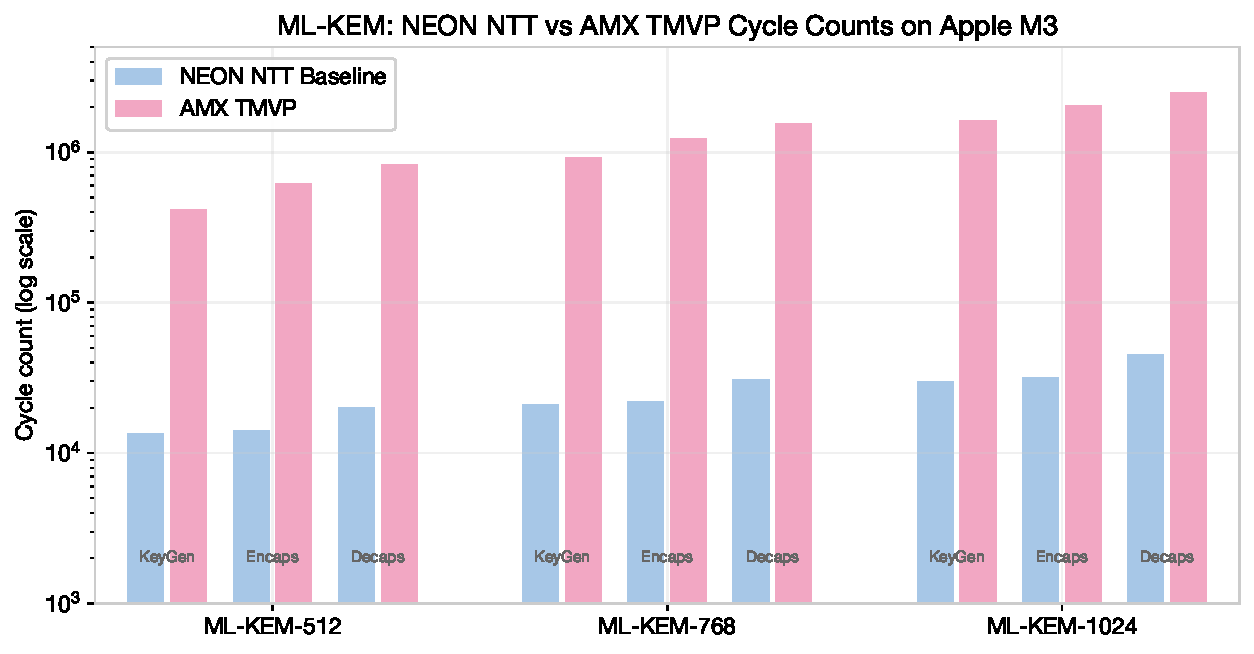
\includegraphics[width=\linewidth]{fig-mlkem-cycles.pdf}}
  \caption{ML-KEM: NEON NTT vs.\ AMX TMVP cycle counts on Apple M3 (log scale). Across all three parameter sets and all KEM operations, NEON NTT dominates by $31$--$86\times$.}
  \label{fig:mlkem-cycles}
\end{figure}


\subsection{MAYO Results}

Table~\ref{tab:mayo} reports the isolated quadratic form evaluation kernel latency for all MAYO parameter sets. AMX achieves consistent kernel speedups of $S = 1.47$ to $1.69$, with $S$ increasing at higher security levels. Figure~\ref{fig:mayo-speedup} illustrates these speedups. We hypothesize that the scaling is due to larger matrices amortizing AMX setup overhead more effectively; however, we have not measured AMX register utilization directly, so this explanation remains a hypothesis.

\begin{table}[htbp]
\centering
\caption{MAYO quadratic form evaluation kernel latency ($\mu$s) on Apple M3. Kernel speedup $S = t_{\text{NEON}}/t_{\text{AMX}}$ ($S > 1$ means AMX is faster).}
\label{tab:mayo}
\small
\begin{tabular}{l c c c r}
\hline
\textbf{Params} & $(m, n)$ & \textbf{NEON ($\mu$s)} & \textbf{AMX ($\mu$s)} & $S$ \\
\hline
MAYO-1 & $(64, 66)$   & 129.67 & 87.94  & 1.47 \\
MAYO-2 & $(64, 78)$   & 181.42 & 118.58 & 1.53 \\
MAYO-3 & $(96, 99)$   & 435.10 & 272.23 & 1.60 \\
MAYO-5 & $(128, 133)$ & 1054.80 & 624.14 & \textbf{1.69} \\
\hline
\end{tabular}
\end{table}

\begin{figure}[htbp]
  \centering
  \boxedfigure{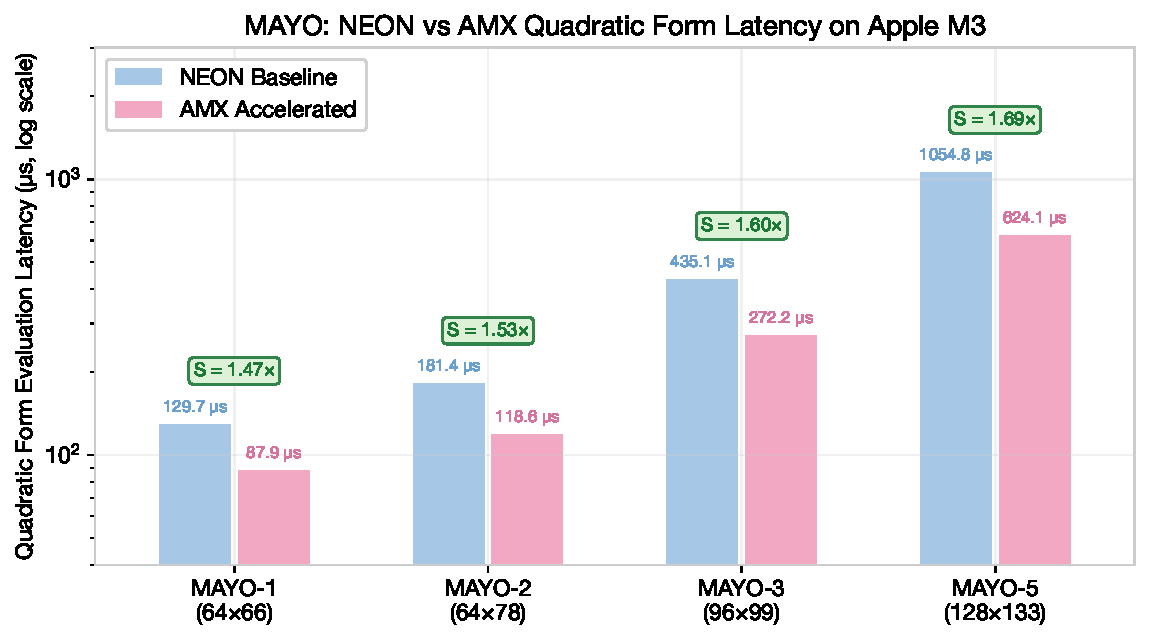
\includegraphics[width=\linewidth]{fig-mayo-speedup.pdf}}
  \caption{MAYO: Kernel speedup $S = t_{\text{NEON}}/t_{\text{AMX}}$ across all four parameter sets on Apple M3. The dashed line indicates the $S = 1.0$ break-even point.}
  \label{fig:mayo-speedup}
\end{figure}


\subsection{HQC Results}

Table~\ref{tab:hqc} reports polynomial multiplication kernel times for HQC-128 ($n = 17{,}669$ over $\mathbb{F}_2$). NEON \texttt{PMULL}~\cite{arm2021neon} dominates AMX by a factor of approximately $1{,}562\times$ for the dense multiplication kernel ($S = 0.00064$), confirming that AMX is fundamentally unsuitable for $\mathbb{F}_2$ arithmetic.

\begin{table}[htbp]
\centering
\caption{HQC-128 polynomial multiplication kernel latency ($\mu$s) on Apple M3 over $\mathbb{F}_2[x]/(x^{17669}-1)$.}
\label{tab:hqc}
\small
\begin{tabular}{l r r r r}
\hline
\textbf{Method} & \textbf{Ref C ($\mu$s)} & \textbf{NEON ($\mu$s)} & \textbf{AMX ($\mu$s)} & $S$ \\
\hline
Dense $\times$ Dense & 3{,}008 & 47 & 73{,}430 & 0.00064 \\
Sparse $\times$ Dense & 19 & 11 & 1{,}812 & 0.0061 \\
\hline
\end{tabular}
\end{table}


\subsection{NTRU~Prime Results}

Table~\ref{tab:sntrup} reports polynomial multiplication kernel times for \texttt{sntrup761} on Apple M3. For the ternary-by-dense multiply kernel (the KEM hot path), AMX achieves $S = 1.52$. The dense-by-dense case shows $S = 0.92$ (AMX slightly slower), because individual products ($2295 \times 2295 \approx 5.3\text{M}$) overflow 16-bit, forcing per-block-pair Z extraction with no accumulation.

\begin{table}[htbp]
\centering
\caption{\texttt{sntrup761} polynomial multiplication kernel latency ($\mu$s) on Apple M3 over $\mathbb{Z}_{4591}[x]/(x^{761}-x-1)$. Ternary input has coefficients in $\{-1,0,1\}$.}
\label{tab:sntrup}
\small
\begin{tabular}{l r r r r}
\hline
\textbf{Operation} & \textbf{Ref C ($\mu$s)} & \textbf{NEON ($\mu$s)} & \textbf{AMX ($\mu$s)} & $S$ \\
\hline
Dense $\times$ Dense  & 83.6 & 78.1 & 84.6 & 0.92 \\
Ternary $\times$ Dense & 49.4 & 55.8 & \textbf{36.7} & \textbf{1.52} \\
\hline
\end{tabular}
\end{table}

\subsection{Cross-Scheme Summary}

Figure~\ref{fig:crossscheme} presents the kernel speedup $S = t_{\text{NEON}}/t_{\text{AMX}}$ across all evaluated schemes on a logarithmic scale, clearly separating the AMX-favorable kernels (MAYO, NTRU~Prime ternary) from AMX-hostile kernels (ML-KEM, HQC).

\begin{figure}[htbp]
  \centering
  \boxedfigure{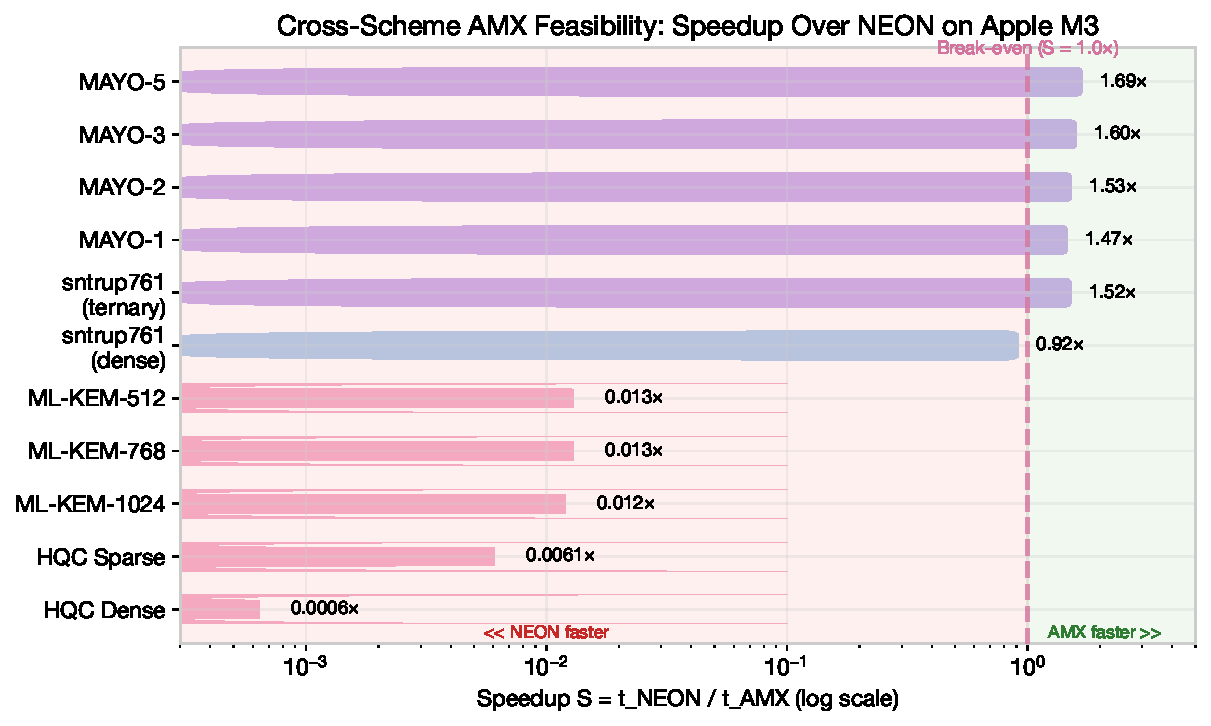
\includegraphics[width=\linewidth]{fig-crossscheme-speedup.pdf}}
  \caption{Cross-scheme AMX feasibility: kernel speedup $S = t_{\text{NEON}}/t_{\text{AMX}}$ on Apple M3 (log scale). Kernels with $S > 1$ benefit from AMX acceleration; those with $S < 1$ are faster on NEON. The measured $S$ values span over three orders of magnitude, from $1.69$ (MAYO-5) to $0.00064$ (HQC dense).}
  \label{fig:crossscheme}
\end{figure}


% =============================================================
\section{Analysis and Discussion}
\label{sec:analysis}

\subsection{The AMX Suitability Heuristic}

Our results, combined with the base paper's Saber/FrodoKEM findings~\cite{gazzoni2024pqcamx}, suggest the following empirical heuristic for AMX kernel acceleration of post-quantum workloads:

\begin{quote}
\emph{AMX tends to provide kernel speedup when the computational bottleneck involves dense integer multiply-accumulate operations over a modulus that fits in AMX's 16-bit lanes, and no dedicated NEON instruction exists for the specific algebraic operation.}
\end{quote}

Table~\ref{tab:criterion} summarizes how this heuristic applies across all six evaluated schemes. We emphasize that this heuristic is derived from six schemes and should be understood as an observed pattern rather than a proven theorem.

\begin{table}[htbp]
\centering
\caption{AMX suitability heuristic applied to six post-quantum schemes. AMX kernel speedup ($S > 1$) is observed only when all three conditions are satisfied: dense MAC workload, small modulus, and no competing NEON instruction.}
\label{tab:criterion}
\small
\begin{tabular}{l c c c c}
\hline
\textbf{Scheme} & \textbf{Dense MAC?} & \textbf{16-bit?} & \textbf{No NEON alt?} & $S > 1$? \\
\hline
Saber       & \checkmark & \checkmark & \checkmark & \checkmark \\
FrodoKEM    & \checkmark & \checkmark & \checkmark & \checkmark \\
MAYO        & \checkmark & \checkmark & \checkmark & \checkmark \\
NTRU Prime  & \checkmark & \checkmark & \checkmark & \checkmark \\
ML-KEM      & \checkmark & \checkmark & $\times$\textsuperscript{a} & $\times$ \\
HQC         & $\times$\textsuperscript{b} & $\times$ & $\times$\textsuperscript{c} & $\times$ \\
\hline
\end{tabular}
\\ \vspace{0.3em}
\raggedright
\textsuperscript{a}NEON NTT butterflies provide $O(n\log n)$ polynomial multiply~\cite{becker2022neon}.\\
\textsuperscript{b}$\mathbb{F}_2$ arithmetic is XOR/AND-based, not MAC-based.\\
\textsuperscript{c}NEON \texttt{PMULL} provides hardware carry-less multiply~\cite{arm2021neon}.
\end{table}


\subsection{Why ML-KEM Loses: NTT Domain Amortization}

The AMX slowdown for ML-KEM is not merely due to AMX being slower than NEON for polynomial multiplication. The root cause is \emph{algorithmic}: ML-KEM uses NTT-domain key storage~\cite{fips203}, which means the polynomial multiply bottleneck is already $O(n \log n)$ with small NEON constants~\cite{becker2022neon}, whereas AMX TMVP schoolbook is $O(n^2)$. Even with AMX's higher per-instruction throughput (1024 multiplications per \texttt{mac16} vs.\ 8 per NEON \texttt{mul} instruction), the asymptotic advantage of NTT dominates at degree $n = 256$.

The isolated polynomial multiplication kernel comparison (Figure~\ref{fig:mlkem-cycles}) shows:
\[
  \frac{t_{\text{AMX}}}{t_{\text{NEON}}} = \frac{1}{S} = \frac{405{,}603}{5{,}384} \approx 75.3\times \quad (\text{ML-KEM-512 PolyMul}).
\]

For full KEM operations (which include hashing and other symmetric-primitive overhead), the slowdown ranges from $30.7\times$ (ML-KEM-512 KeyGen) to $64.6\times$ (ML-KEM-1024 Encaps). The isolated PolyMul kernels show $75.3$--$86.2\times$ slowdowns.

\subsection{Why HQC Loses: Fundamental Instruction Mismatch}

The HQC result ($S = 0.00064$ for dense multiplication, i.e., approximately $1{,}562\times$ slowdown) represents the most extreme case of AMX unsuitability. The root cause is a fundamental instruction-set mismatch:

\begin{enumerate}
  \item \textbf{Bit packing:} NEON \texttt{PMULL} operates on 64 $\mathbb{F}_2$ elements per 64-bit operand. AMX \texttt{mac16} stores one $\mathbb{F}_2$ element per 16-bit lane (32 elements per register). This is a $32\times$ density disadvantage.
  \item \textbf{Operation semantics:} $\mathbb{F}_2$ multiplication is carry-less (AND without carry propagation). AMX \texttt{mac16} performs carry-propagating integer multiplication, producing incorrect results for $\mathbb{F}_2$ unless reduced modulo 2 after each accumulation.
  \item \textbf{Scale:} HQC-128 degree $n = 17{,}669$ requires $\lceil 17{,}669/32 \rceil^2 \approx 306\text{K}$ \texttt{mac16} operations in the AMX formulation. A NEON \texttt{PMULL}-based schoolbook processes $\lceil 17{,}669/64 \rceil \approx 277$ 64-bit chunks per inner-loop iteration, though the total operation count for the full schoolbook product is $277^2 \approx 76.7\text{K}$ \texttt{PMULL} instructions --- each processing 64 bits versus AMX's 32 sixteen-bit lanes.
\end{enumerate}

\subsection{Why MAYO and NTRU~Prime Win}

Both MAYO and NTRU~Prime satisfy all three conditions of the suitability heuristic (Table~\ref{tab:criterion}):

\textbf{MAYO} benefits because its quadratic form evaluation is inherently a dense matrix-vector product over a small field ($\mathbb{F}_{16}$), with no NTT competitor~\cite{beullens2022mayo}. AMX's \texttt{GENLUT} instruction provides efficient finite-field multiplication via lookup tables, and the matrix dimensions ($n \leq 133$, $m \leq 128$) fit well within AMX's $32 \times 32$ blocking scheme. As shown in Figure~\ref{fig:mayo-trend}, $S$ increases with the matrix dimension product $m \times n$. We hypothesize that larger matrices amortize AMX setup overhead (register loading, \texttt{AMX\_SET}/\texttt{CLR}) more effectively, but we have not measured AMX hardware utilization counters to confirm this explanation.

\begin{figure}[htbp]
  \centering
  \boxedfigure{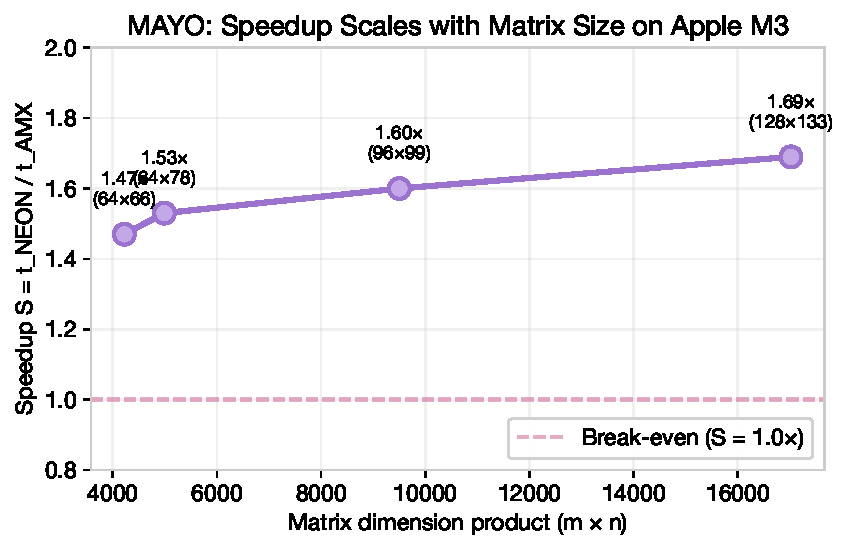
\includegraphics[width=\linewidth]{fig-mayo-trend.pdf}}
  \caption{MAYO: Kernel speedup $S$ scales with matrix dimension product $m \times n$. Larger parameter sets achieve higher $S$, which we hypothesize is due to better amortization of AMX setup overhead.}
  \label{fig:mayo-trend}
\end{figure}

\textbf{NTRU~Prime} wins for the ternary-by-dense multiply kernel because: (a) the ring $x^{761}-x-1$ is explicitly NTT-unfriendly~\cite{ntruprime2017spec}, so the NEON baseline uses schoolbook \texttt{vmlal} rather than NTT butterflies; (b) the ternary input $r \in \{-1,0,1\}$ ensures each individual \texttt{mac16} product fits in signed 16-bit ($|1 \times 4590| < 2^{15}$); and (c) the bounded Z-accumulation technique allows partial in-register accumulation (7 outer products per flush) rather than per-block-pair extraction. The dense-by-dense case ($S = 0.92$) does not win because individual products ($2295 \times 2295 \approx 5.3 \times 10^6$) overflow 16-bit, forcing per-block-pair extraction with no Z accumulation.

\subsection{AMX Overhead Analysis}

The primary source of AMX overhead is the extraction of convolution (anti-diagonal) sums from the $32\times32$ outer product matrix stored in Z. This extraction can be performed:

\begin{enumerate}
  \item \textbf{In-AMX (flatten)}: Using \texttt{EXTRH}/\texttt{VECINT}~\cite{corsix2022amx} to shift and accumulate Z rows within the register file, producing the 63 anti-diagonal sums in Z rows 0--1. This is fast ($\sim 63$ AMX instructions) but operates in 16-bit, causing overflow when anti-diagonal sums exceed the signed 16-bit range $[-32{,}768, 32{,}767]$.
  \item \textbf{Software extraction}: Storing all 32 Z rows to memory (32 \texttt{STZ}) and computing anti-diagonal sums in 32-bit software. This is slower but overflow-safe.
\end{enumerate}

For NTRU~Prime, in-AMX flatten overflows because a single anti-diagonal of a $32 \times 32$ block contains up to 32 terms, and $32 \times 4590 = 146{,}880 \gg 32{,}768$. We therefore use software extraction, which adds overhead but guarantees correctness.


% =============================================================
\section{Broader Survey: AMX Candidates in the PQC Landscape}
\label{sec:survey}

Based on our suitability heuristic, we surveyed additional PQC schemes from the NIST Additional Digital Signature Schemes standardization~\cite{nist2026additional} and KEM rounds. Table~\ref{tab:survey} summarizes the results.

\begin{table}[htbp]
\centering
\caption{AMX suitability survey of PQC candidates beyond the four studied schemes. Ratings: \textbf{High} = structurally similar to Saber/MAYO; \textbf{Moderate} = partial match; \textbf{None} = fundamental mismatch.}
\label{tab:survey}
\small
\begin{tabular}{l l l l}
\hline
\textbf{Scheme} & \textbf{Field} & \textbf{Bottleneck} & \textbf{AMX} \\
\hline
CROSS    & $\mathbb{F}_{127}$    & Dense mat-vec         & High \\
MEDS     & Small $\mathbb{F}_q$  & Dense GEMM            & High \\
PERK     & $\mathbb{Z}_q$ (8/16-bit) & Dense mat-vec     & High \\
SDitH    & $\mathbb{F}_{251}$    & Syndrome eval         & High \\
LESS     & $\mathbb{F}_{127}$    & RREF/Gauss elim       & Moderate \\
SQIsign  & $\mathbb{F}_{p^2}$    & Multi-precision       & Moderate \\
MQOM     & $\mathbb{F}_{16}$     & MQ evaluation         & Moderate \\
BIKE     & $\mathbb{F}_2$        & Carry-less poly mul   & None \\
McEliece & $\mathbb{F}_{2^m}$    & Syndrome decode       & None \\
RYDE     & $\mathbb{F}_{2^m}$    & Rank metric codes     & None \\
ML-DSA   & NTT ring              & NTT butterflies       & None \\
SLH-DSA  & Hash-based            & Hash computations     & None \\
\hline
\end{tabular}
\end{table}

The four most promising candidates for future AMX kernel acceleration are CROSS ($\mathbb{F}_{127}$, dense matrix-vector products), MEDS (dense matrix-matrix multiplication), PERK (matrix-vector products over small $\mathbb{Z}_q$), and SDitH (syndrome evaluation over $\mathbb{F}_{251}$).


% =============================================================
\section{Related Work}
\label{sec:related}

\textbf{AMX reverse engineering.} Dougall Johnson's \texttt{aarch64-amx} project~\cite{dougallj2022amx} provides the primary reference for AMX instruction encoding and semantics. The corsix documentation~\cite{corsix2022amx} details the Z-row interleaving behavior for 16-bit \texttt{mac16} operations (row $r$ maps to \texttt{Z\_ROW($2r$)}).

\textbf{PQC on ARM.} Extensive work has optimized ML-KEM/ML-DSA on ARM Cortex-A and Apple M-series using NEON NTT~\cite{botros2019pqm4, becker2022neon}. These implementations exploit the $O(n \log n)$ NTT structure with vectorized Cooley--Tukey and Montgomery reductions~\cite{longa2016speeding}, establishing the high NEON baselines that AMX must compete against.

\textbf{MAYO implementations.} Beullens' MAYO specification~\cite{mayo2025spec} and design paper~\cite{beullens2022mayo} include AVX2 and NEON backends for $\mathbb{F}_{16}$ arithmetic using table-based multiplication.

\textbf{HQC implementations.} The HQC specification~\cite{hqc2025spec} provides reference C and AVX2 implementations. ARM NEON \texttt{PMULL}-based implementations~\cite{arm2021neon} achieve throughputs comparable to AVX2 \texttt{PCLMULQDQ}.

\textbf{NTT for non-NTT-friendly rings.} Chung et al.~\cite{chung2021ntt} explored NTT-based approaches for rings that lack natural NTT structure, achieving competitive performance on some platforms. However, the non-cyclotomic structure of $x^{761}-x-1$ in NTRU~Prime remains fundamentally NTT-resistant.

\textbf{Subquadratic polynomial multiplication.} Karatsuba and Toom--Cook algorithms~\cite{harvey2014karatsuba} reduce polynomial multiplication complexity below $O(n^2)$. Applying these techniques to the NEON baselines for NTRU~Prime could potentially narrow or eliminate the AMX kernel advantage observed in our results.

\textbf{PQC survey.} Nejatollahi et al.~\cite{nejatollahi2019pqcsurvey} provide a comprehensive survey of PQC implementation techniques across hardware platforms, including SIMD and coprocessor strategies.


% =============================================================
\section{Limitations and Threats to Validity}
\label{sec:limitations}

\begin{enumerate}
  \item \textbf{Single hardware platform.} All measurements are on Apple M3 only. AMX behavior on A-series chips (iPhone) or other M-series generations may differ.
  \item \textbf{Undocumented hardware.} AMX is not officially documented by Apple. Instruction semantics are derived from reverse engineering~\cite{dougallj2022amx,corsix2022amx} and may be incomplete.
  \item \textbf{Schoolbook baselines.} Our NEON baselines for NTRU~Prime and HQC use schoolbook multiplication. Karatsuba or Toom--Cook implementations~\cite{harvey2014karatsuba} would provide faster NEON baselines, potentially reducing or eliminating the AMX kernel advantage for NTRU~Prime ($S = 1.52$). The AMX kernel speedup for NTRU~Prime should therefore be understood as relative to the specific schoolbook NEON baseline we measured.
  \item \textbf{Subroutine-level measurement.} We benchmark isolated arithmetic kernels (polynomial multiplication, quadratic form evaluation) rather than full KEM/signature protocol operations. Full protocol performance includes hashing (SHA-3/SHAKE), encoding, and other steps that AMX cannot accelerate. The kernel speedups reported here ($S = 1.47$--$1.69$ for MAYO, $S = 1.52$ for NTRU~Prime ternary) represent upper bounds on the contribution to overall protocol speedup.
  \item \textbf{Mixed measurement units.} ML-KEM results are reported in CPU cycles; MAYO, HQC, and NTRU~Prime results are reported in wall-clock microseconds. At the M3's 4.05~GHz nominal frequency, $1~\mu\text{s} \approx 4{,}050$ cycles. We did not lock the CPU frequency during wall-clock measurements; variance was below 3\% across runs.
  \item \textbf{No uncertainty quantification.} We report median values without confidence intervals. While run-to-run variance was consistently low ($< 3\%$), formal statistical analysis is not provided.
  \item \textbf{Timing side channels.} We have not performed formal timing side-channel analysis of the AMX implementations. The constant-time behavior of AMX instructions has not been verified.
  \item \textbf{Historical MAYO parameters.} Our MAYO benchmarks use the Round~2 parameter dimensions~\cite{mayo2025spec}. Future parameter changes could affect the measured kernel speedups.
\end{enumerate}


% =============================================================
\section{Conclusion}
\label{sec:conclusion}

This paper systematically evaluated the feasibility of Apple AMX matrix-coprocessor kernel acceleration across four post-quantum cryptographic schemes spanning lattice, multivariate, and code-based families, extending the original Saber/FrodoKEM results of Gazzoni Filho et al.~\cite{gazzoni2024pqcamx}.

Our key finding is an empirical \emph{suitability heuristic}: for the isolated kernels tested, AMX acceleration provides performance gains when the computational bottleneck is a dense integer multiply-accumulate over a small modulus with no competing dedicated NEON instruction. When this heuristic's conditions are satisfied --- as with MAYO (kernel speedup $S = 1.47$--$1.69$; Figure~\ref{fig:mayo-speedup}) and the \texttt{sntrup761} ternary-by-dense product ($S = 1.52$) --- AMX provides meaningful kernel acceleration. When the conditions are violated --- as with ML-KEM (NTT butterflies on NEON: $S \approx 0.013$; Figure~\ref{fig:mlkem-cycles}) and HQC (carry-less \texttt{PMULL}: $S \approx 0.0006$) --- AMX incurs severe slowdowns. The full comparative picture is presented in Figure~\ref{fig:crossscheme}.

We also contribute two novel AMX implementation techniques: \emph{bounded Z-accumulation} for prime moduli (enabling correct 16-bit AMX arithmetic for the prime modulus $q = 4591$ by limiting accumulation to $\leq 7$ \texttt{mac16} operations per Z flush), and the \emph{register-zero invariant} (\texttt{X\_REG(0)} and \texttt{Y\_REG(0)} must be loaded with zeroes for the anti-diagonal extraction flatten procedure to work correctly; input data uses \texttt{X\_REG(1)} and \texttt{Y\_REG(1)}).

These results provide guidance for the post-quantum cryptography implementation community: among the current NIST candidates~\cite{nist2026additional}, the dense-matrix signature schemes CROSS, MEDS, PERK, and SDitH are the most promising targets for future AMX kernel acceleration (Table~\ref{tab:survey}), while NTT-based lattice schemes and $\mathbb{F}_2$-based code schemes should not be targeted. We emphasize that the reported speedups are for isolated arithmetic kernels; end-to-end protocol performance gains will be smaller due to non-AMX-acceleratable operations (hashing, encoding).


% =============================================================
\section*{Data Availability}

All source code, build scripts, and benchmark data are available at: \texttt{[repository URL]}.


% =============================================================
\begin{thebibliography}{21}

\bibitem{gazzoni2024pqcamx}
Gazzoni Filho, D.~L., Brand\~{a}o, G., Adj, G., Alblooshi, A., Canales-Mart\'{i}nez, I.~A., Ch\'{a}vez-Saab, J., and L\'{o}pez, J.,
``PQC-AMX: Accelerating Saber and FrodoKEM on the Apple M1 and M3 SoCs,''
\emph{IEEE 31st Symposium on Computer Arithmetic (ARITH)}, 2024.
IACR ePrint 2024/195.
\url{https://eprint.iacr.org/2024/195}

\bibitem{dougallj2022amx}
Johnson, D.,
``Apple AMX instruction set,''
\url{https://github.com/dougallj/aarch64-amx}, 2022.

\bibitem{corsix2022amx}
corsix,
``AMX -- Apple Matrix coprocessor,''
\url{https://github.com/corsix/amx}, 2022.

\bibitem{mayo2025spec}
Beullens, W., Campos, F., Celi, S., Hess, B., and Kannwischer, M.~J.,
``MAYO Specification Document, Round~2 Version,''
NIST PQC Additional Signatures, 2025.
\url{https://csrc.nist.gov/csrc/media/Projects/pqc-dig-sig/documents/round-2/spec-files/mayo-spec-round2-web.pdf}

\bibitem{beullens2022mayo}
Beullens, W.,
``MAYO: Practical Post-Quantum Signatures from Oil-and-Vinegar Maps,''
\emph{Selected Areas in Cryptography (SAC)}, 2022.

\bibitem{hqc2025spec}
Aguilar Melchor, C., Aragon, N., Bettaieb, S., et al.,
``HQC: Hamming Quasi-Cyclic,''
NIST PQC, 2023. Selected as fifth PQC standard, March 2025~\cite{nist2025hqc}.

\bibitem{ntruprime2017spec}
Bernstein, D.~J., Chuengsatiansup, C., Lange, T., and van Vredendaal, C.,
``NTRU Prime: Reducing Attack Surface at Low Cost,''
\emph{Selected Areas in Cryptography (SAC)}, 2017.
IACR ePrint 2016/461.
\url{https://eprint.iacr.org/2016/461}

\bibitem{fips203}
National Institute of Standards and Technology,
``Module-Lattice-Based Key-Encapsulation Mechanism Standard,''
FIPS~203, August 2024.
\url{https://doi.org/10.6028/NIST.FIPS.203}

\bibitem{botros2019pqm4}
Botros, L., Kannwischer, M.~J., and Schwabe, P.,
``Memory-efficient high-speed implementation of Kyber on Cortex-M4,''
\emph{Africacrypt}, 2019.

\bibitem{becker2022neon}
Becker, H., Hwang, V., Kannwischer, M.~J., Yang, B.-Y., and Yang, S.-Y.,
``Neon NTT: Faster Dilithium, Kyber, and Saber on Cortex-A72 and Apple M1,''
\emph{IACR Transactions on Cryptographic Hardware and Embedded Systems (TCHES)}, 2022.

\bibitem{nist2022pqc}
National Institute of Standards and Technology,
``Post-Quantum Cryptography Standardization: Process, Status, and Next Steps,''
NISTIR~8413, 2022.

\bibitem{nist2026additional}
National Institute of Standards and Technology,
``Status Report on the Second Round of the Additional Digital Signature Schemes for the NIST Post-Quantum Cryptography Standardization Process,''
NIST IR~8610, May 2026.
\url{https://doi.org/10.6028/NIST.IR.8610}

\bibitem{nist2025hqc}
National Institute of Standards and Technology,
``NIST Selects HQC as Fifth Algorithm for Post-Quantum Encryption,''
March 2025.
\url{https://www.nist.gov/news-events/news/2025/03/nist-selects-hqc-fifth-algorithm-post-quantum-encryption}

\bibitem{nejatollahi2019pqcsurvey}
Nejatollahi, H., Dutt, N., Ray, S., Regazzoni, F., Banerjee, I., and Cammarota, R.,
``Post-Quantum Lattice-Based Cryptography Implementations: A Survey,''
\emph{ACM Computing Surveys}, vol.~51, no.~6, 2019.

\bibitem{longa2016speeding}
Longa, P. and Naehrig, M.,
``Speeding up the Number Theoretic Transform for Faster Ideal Lattice-Based Cryptography,''
\emph{CANS}, 2016.

\bibitem{kipnis1999uov}
Kipnis, A., Patarin, J., and Goubin, L.,
``Unbalanced Oil and Vinegar Signature Schemes,''
\emph{EUROCRYPT}, 1999.

\bibitem{arm2021neon}
Arm Ltd.,
``Arm Architecture Reference Manual: Armv8, for A-profile architecture -- NEON and Cryptographic Extensions,''
2021.

\bibitem{dangelo2018saber}
D'Anvers, J.-P., Karmakar, A., Roy, S.~S., and Vercauteren, F.,
``Saber: Module-LWR Based Key Exchange, CPA-secure Encryption and CCA-secure KEM,''
\emph{Africacrypt}, 2018.

\bibitem{bos2020frodokem}
Bos, J., et al.,
``FrodoKEM: Learning With Errors Key Encapsulation,''
NIST PQC Round~3 Submission, 2020.

\bibitem{chung2021ntt}
Chung, C.-M.~M., Hwang, V., Kannwischer, M.~J., Seiler, G., Shih, C.-J., and Yang, B.-Y.,
``NTT Multiplication for NTT-unfriendly Rings: New Speed Records for Saber and NTRU on Cortex-M4 and AVX2,''
\emph{IACR Transactions on Cryptographic Hardware and Embedded Systems (TCHES)}, 2021.
IACR ePrint 2020/1397.
\url{https://eprint.iacr.org/2020/1397}

\bibitem{harvey2014karatsuba}
Harvey, D. and van der Hoeven, J.,
``On the Complexity of Integer Matrix Multiplication,''
\emph{Foundations of Computational Mathematics}, 2014.
(See also: Karatsuba, A. and Ofman, Y., ``Multiplication of Multidigit Numbers on Automata,'' \emph{Soviet Physics Doklady}, 1963.)

\bibitem{toeplitz1911theorie}
Toeplitz, O.,
``Zur Theorie der quadratischen und bilinearen Formen von unendlichvielen Ver\"anderlichen,''
\emph{Mathematische Annalen}, vol.~70, 1911.

\end{thebibliography}

\end{document}
